\documentclass[11pt]{article}

\usepackage[T1]{fontenc}
\usepackage{lmodern}
\usepackage[margin=1in]{geometry}
\usepackage{microtype}
\usepackage{amsmath,amssymb,mathtools}
\usepackage{booktabs,longtable,array}
\usepackage{graphicx}
\usepackage{pdflscape}
\usepackage{enumitem}
\usepackage{xcolor}
\usepackage{caption}
\usepackage{placeins}
\usepackage[colorlinks=true,
            linkcolor=blue!55!black,
            urlcolor=blue!55!black,
            citecolor=blue!55!black]{hyperref}

\setlength{\parindent}{0pt}
\setlength{\parskip}{0.55em}
\setlength{\emergencystretch}{3em}
\setlist{itemsep=0.25em,topsep=0.35em}
\captionsetup{font=small,labelfont=bf}
\renewcommand{\arraystretch}{1.16}

\newcommand{\ii}{\mathrm{i}}
\newcommand{\A}{\mathcal{A}}
\newcommand{\cI}{\mathcal{I}}
\newcommand{\QMC}{\mathrm{QMC}}

\title{Torus \texorpdfstring{$1\to n$}{1 to n} Amplitudes in the
       \texorpdfstring{$c=1$}{c=1} String\\[0.4em]
       \large A numerical worldsheet note}
\author{}
\date{25 August 2026}

\begin{document}
\maketitle

\begin{abstract}
This note records the current numerical worldsheet results for torus
$1\to n$ tachyon amplitudes in the $c=1$ string.  The genus-one $1\to1$
reflection amplitude is evaluated at fifty points on the imaginary-energy
ray $\omega=\ii t$, $0<t<1$.  Its torus two-point block uses necklace
internal-weight recursion away from collision, OPE central-charge recursion
near collision, and exact finite-level descendant sewing as an audited
fallback.  The native worldsheet data are frozen before the BRY convention
map and matrix-model comparison are applied.  A correlated fifty-point fit
gives
\begin{equation*}
 (a,b,c)=(1.0016588,1.0053852,1.0093253),
 \qquad \kappa=1.0082693,
\end{equation*}
with shared-scramble RQMC uncertainties stated below.  The genus-one
$1\to2$ amplitude is now represented only by its current target-blind
ten-point equal-split scan in the pole-free strip.  It uses order-eight
momentum quadrature, an $h$-recursion-dominant channel atlas with necklace
orders $(8,3,3)$, and $c$-recursion only in the small OPE patches.  After the
worldsheet scan and its shape analysis were separately frozen, all ten points
were found within one quoted RQMC standard error of the BRY-normalized
matrix-model curve.  No claim at general multiplicity is inferred.
\end{abstract}

\tableofcontents

\section{Scope and status}
\label{sec:scope}

There are two numerical claims and one explicit limitation in this note.
\begin{enumerate}
  \item The torus $1\to1$ amplitude has a frozen fifty-point worldsheet scan
  with $0.02\leq t\leq0.99$.  All points use one common hybrid-recursion,
  momentum-quadrature, cutoff, tail, and shared-scramble design.  The complete
  native dataset was frozen before the BRY notation map or matrix-model
  comparison was applied.  Sections~\ref{sec:two-point-design}--
  \ref{sec:two-point-limitations} contain only this current result.

  \item The torus $1\to2$ amplitude has a frozen target-blind ten-point scan
  at equal split and $0.05\leq t\leq0.95$.  Every point uses the same
  momentum-order-eight, $h$-recursion-dominant channel atlas and four aligned
  RQMC scrambles.  The bulk region and the direct importance-sampled tail to
  $\tau_2=\infty$ are integrated in one run.  The worldsheet shape analysis
  was frozen before the BRY-normalized matrix curve was evaluated.

  \item No general torus $1\to n$ formula is inferred from either calculation.
  The two-point and three-point moduli integrals have different dimensions,
  block structures, and numerical systematics.
\end{enumerate}

The order of operations is fixed throughout: analytically continue to the
convergent imaginary-energy chamber, evaluate and serialize the worldsheet
integral without importing a target polynomial, freeze the native artifacts,
and only then transform conventions or compare with target-space data.  The
production artifacts record this trust boundary explicitly.

\section{Worldsheet and BRY conventions}
\label{sec:conventions}

From this point onward, \(g_s\) denotes the BRY string coupling.  Thus
\begin{equation}
 \boxed{\mu^{-1}=2\pi g_s.}
 \label{eq:bry-coupling-dictionary}
\end{equation}
The older string-note coupling is not used below; when comparison with a
legacy artifact is unavoidable it is related by
\(g_s=2g_s^{\mathrm{SN}}\).

For the torus two-point function, the target-free sewing normalization is
\begin{equation}
 \boxed{
 \A^{\mathrm{ws}}_1(\omega)
 =2\pi^2\ii g_s^2\,\cI_1(\omega).}
 \label{eq:two-point-native}
\end{equation}
Only after the native calculation is frozen, the BRY coupling dictionary
gives~\cite{BRY}
\begin{equation}
 \boxed{
 -\ii\A_{1\to1}^{(1)}(\ii t)=\frac{1}{2}\cI_1(\ii t).}
 \label{eq:two-point-bry-map}
\end{equation}
The external Liouville weight and internal weights are
\begin{equation}
 d=1+\frac{\omega^2}{4},
 \qquad h(P)=1+P^2.
\end{equation}
For $\omega=\ii t$ with $0<t<1$, no DOZZ pole crosses a positive-real
internal-momentum contour.  The moduli integral is directly convergent: no
physical-domain subtraction or crossed-pole residue enters the fifty-point
dataset.

For the torus three-point calculation, the native and stripped normalizations
used below are
\begin{equation}
 \A^{\mathrm{ws}}_{1,3}
 =2\pi^2\ii g_s^3\cI_{1,3},
 \qquad
 F_1^{\mathrm{ws}}=\frac{\cI_{1,3}}{4\pi}.
 \label{eq:three-point-normalization}
\end{equation}

\section{Current fifty-point \texorpdfstring{$1\to1$}{1 to 1}
hybrid-recursion design}
\label{sec:two-point-design}

The punctured torus is split at $\epsilon=0.15$.  For the nearest lattice
representative satisfying
\begin{equation}
 |z_{\mathrm{local}}|<2\pi\epsilon,
\end{equation}
the OPE channel uses
\begin{equation}
 q=\exp(2\pi\ii\tau),
 \qquad
 v=\exp(-\ii z_{\mathrm{local}})-1,
 \label{eq:ope-coordinates}
\end{equation}
and fixed-weight central-charge recursion through orders
$(N_q,N_v)=(3,8)$.  Its flat-frame primary factor remains
\begin{equation}
 q^{h_{\mathrm{loop}}-25/24}v^{h_{\mathrm{OPE}}}
 \bigl[2\sin(z_{\mathrm{local}}/2)\bigr]^{-2d}.
 \label{eq:ope-primary-factor}
\end{equation}
The recursion changes only the descendant-coefficient generator and
introduces no additional Weyl factor.

Away from collision, the necklace channel uses simultaneous internal-weight
recursion through orders $(6,3)$.  Resonant terms at $c=25$ are defined by a
three-point Richardson limit in $c\to25$ with production regulator
$\delta c=0.04$, and by a symmetric generic-weight limit at confluent poles
with $\delta h=10^{-3}$.  Every coefficient tensor is independently audited
at tolerance $10^{-7}$; failed nodes use exact finite-level descendant
sewing.

The common numerical design is:
\begin{itemize}
  \item four scrambled Sobol replicas with $2^8=256$ four-dimensional points
  per cutoff;
  \item bulk cutoffs $\tau_2=3,4,6,8$;
  \item four tail replicas with $2^7=128$ points per slice at
  $\tau_2=8,10,12,16,20$;
  \item the tail ansatz
  $f(\tau_2)=a_0\tau_2^{-2}+a_1\tau_2^{-5/3}+a_2\tau_2^{-3}$;
  \item two 16-point Gauss--Legendre momentum integrals with $P_{\max}=6$
  and threshold-resolving map $P=6u^2$;
  \item collision-disc radius $0.10$, with the leading OPE contribution
  integrated analytically;
  \item the same four scramble labels at all fifty energies.
\end{itemize}

The hybrid evaluator agrees with a complete direct-descendant rerun at
$t=0.45$ to $2.07\times10^{-13}$ in $\cI_1$, or
$1.80\times10^{-11}$ relatively.  OPE $c$-recursion coefficients through
$(q^4,v^5)$ agree with direct coefficients to $1.35\times10^{-14}$ at generic
weights and $3.6\times10^{-12}$ at coincident internal weights.

\clearpage
\section{Frozen fifty-point \texorpdfstring{$1\to1$}{1 to 1} dataset}
\label{sec:two-point-data}

The quoted errors are the standard errors of the four shared-scramble RQMC
means.  They do not include block-order, momentum, collision-disc, or
cusp-tail model systematics.  The two halves of the energy grid are displayed
side by side in Table~\ref{tab:two-point-data}.

\begin{table}[htbp]
\centering
\caption{Current frozen fifty-point native worldsheet dataset.}
\label{tab:two-point-data}
\small
\resizebox{\textwidth}{!}{%
\begin{tabular}{r r r @{}c@{\hspace{2em}} r r r}
\toprule
$t$ & $\cI_1(\ii t)$ & $\sigma_{\QMC}$ &&
$t$ & $\cI_1(\ii t)$ & $\sigma_{\QMC}$\\
\midrule
0.02 & $-3.35971048\times10^{-5}$ & $1.62\times10^{-6}$ && 0.52 & $-1.34500776\times10^{-2}$ & $7.96\times10^{-4}$\\
0.04 & $-1.34062367\times10^{-4}$ & $6.47\times10^{-6}$ && 0.54 & $-1.38822705\times10^{-2}$ & $8.30\times10^{-4}$\\
0.05 & $-2.09091786\times10^{-4}$ & $1.01\times10^{-5}$ && 0.55 & $-1.40756228\times10^{-2}$ & $8.46\times10^{-4}$\\
0.07 & $-4.07841860\times10^{-4}$ & $1.98\times10^{-5}$ && 0.57 & $-1.44134033\times10^{-2}$ & $8.75\times10^{-4}$\\
0.10 & $-8.23862706\times10^{-4}$ & $4.02\times10^{-5}$ && 0.60 & $-1.47879798\times10^{-2}$ & $9.10\times10^{-4}$\\
0.12 & $-1.17600960\times10^{-3}$ & $5.76\times10^{-5}$ && 0.62 & $-1.49424840\times10^{-2}$ & $9.26\times10^{-4}$\\
0.14 & $-1.58428488\times10^{-3}$ & $7.80\times10^{-5}$ && 0.64 & $-1.50155537\times10^{-2}$ & $9.37\times10^{-4}$\\
0.15 & $-1.80833205\times10^{-3}$ & $8.93\times10^{-5}$ && 0.65 & $-1.50202590\times10^{-2}$ & $9.40\times10^{-4}$\\
0.17 & $-2.29374374\times10^{-3}$ & $1.14\times10^{-4}$ && 0.67 & $-1.49636491\times10^{-2}$ & $9.40\times10^{-4}$\\
0.20 & $-3.10697282\times10^{-3}$ & $1.56\times10^{-4}$ && 0.70 & $-1.47074092\times10^{-2}$ & $9.26\times10^{-4}$\\
0.22 & $-3.69904326\times10^{-3}$ & $1.87\times10^{-4}$ && 0.72 & $-1.44181503\times10^{-2}$ & $9.07\times10^{-4}$\\
0.24 & $-4.32522823\times10^{-3}$ & $2.21\times10^{-4}$ && 0.74 & $-1.40314033\times10^{-2}$ & $8.78\times10^{-4}$\\
0.25 & $-4.64947974\times10^{-3}$ & $2.39\times10^{-4}$ && 0.75 & $-1.38008957\times10^{-2}$ & $8.60\times10^{-4}$\\
0.27 & $-5.31691750\times10^{-3}$ & $2.75\times10^{-4}$ && 0.77 & $-1.32647535\times10^{-2}$ & $8.17\times10^{-4}$\\
0.30 & $-6.35490981\times10^{-3}$ & $3.34\times10^{-4}$ && 0.80 & $-1.22712081\times10^{-2}$ & $7.35\times10^{-4}$\\
0.32 & $-7.06305135\times10^{-3}$ & $3.75\times10^{-4}$ && 0.82 & $-1.14822848\times10^{-2}$ & $6.68\times10^{-4}$\\
0.34 & $-7.77718831\times10^{-3}$ & $4.17\times10^{-4}$ && 0.84 & $-1.05925320\times10^{-2}$ & $5.93\times10^{-4}$\\
0.35 & $-8.13461085\times10^{-3}$ & $4.39\times10^{-4}$ && 0.85 & $-1.01100702\times10^{-2}$ & $5.52\times10^{-4}$\\
0.37 & $-8.84631647\times10^{-3}$ & $4.82\times10^{-4}$ && 0.87 & $-9.07045177\times10^{-3}$ & $4.65\times10^{-4}$\\
0.40 & $-9.89432405\times10^{-3}$ & $5.48\times10^{-4}$ && 0.90 & $-7.32536319\times10^{-3}$ & $3.27\times10^{-4}$\\
0.42 & $-1.05707747\times10^{-2}$ & $5.92\times10^{-4}$ && 0.92 & $-6.04013651\times10^{-3}$ & $2.35\times10^{-4}$\\
0.44 & $-1.12220612\times10^{-2}$ & $6.36\times10^{-4}$ && 0.94 & $-4.66456393\times10^{-3}$ & $1.48\times10^{-4}$\\
0.45 & $-1.15362905\times10^{-2}$ & $6.57\times10^{-4}$ && 0.95 & $-3.94632373\times10^{-3}$ & $1.09\times10^{-4}$\\
0.47 & $-1.21379894\times10^{-2}$ & $6.99\times10^{-4}$ && 0.97 & $-2.43769807\times10^{-3}$ & $4.36\times10^{-5}$\\
0.50 & $-1.29619911\times10^{-2}$ & $7.59\times10^{-4}$ && 0.99 & $-8.36996171\times10^{-4}$ & $5.13\times10^{-6}$\\
\bottomrule
\end{tabular}}
\end{table}

The canonical manifest is
\begin{center}
\path{results/genus1_two_point_worldsheet/imaginary_hybrid_hc_t_scan10_n256_v2/worldsheet_scan_manifest.json}.
\end{center}
It records the fifty source paths, hashes, native values, errors, four
replicas, cutoff sequence, tail slices, and common numerical design.

\section{Current fifty-point fit and analytic comparison}
\label{sec:two-point-fit}

Only after freezing the native data, all fifty values are mapped through
\eqref{eq:two-point-bry-map} and fitted to the BRY ansatz
\begin{equation}
 -\ii\A_{1\to1}^{(1)}(\ii t)
 =\frac{-a t^2+2b t^4-c t^5}{24}.
 \label{eq:two-point-fit-ansatz}
\end{equation}
The RQMC-error-weighted fit is
\begin{equation}
 \boxed{
 a=1.0016588\pm0.0565665,\quad
 b=1.0053852\pm0.0666207,\quad
 c=1.0093253\pm0.0764546.}
 \label{eq:two-point-fit}
\end{equation}
The errors are obtained by fitting each of the four complete shared-scramble
curves.  The coefficients are strongly correlated.  Imposing the analytic
shape $a=b=c=\kappa$ gives
\begin{equation}
 \boxed{\kappa=1.0082693\pm0.0240434.}
 \label{eq:two-point-kappa}
\end{equation}
The raw pointwise worldsheet/matrix-model ratios range from $0.99165$ to
$1.01474$.

The matrix-model prediction in BRY notation is
\begin{equation}
 -\ii\A_{1\to1,\mathrm{MM}}^{(1)}(\ii t)
 =\frac{-t^2+2t^4-t^5}{24},
 \qquad (a,b,c)_{\mathrm{MM}}=(1,1,1).
 \label{eq:two-point-matrix-model}
\end{equation}
BRY reported $(a,b,c)=(1.018,1.028,1.0344)$~\cite{BRY}.  The direct
comparison is shown in Table~\ref{tab:bry-comparison}.

\begin{table}[htbp]
\centering
\caption{Current fifty-point fit compared with the exact matrix-model
coefficients and the BRY numerical fit.}
\label{tab:bry-comparison}
\begin{tabular}{c c c c c}
\toprule
coefficient & matrix model & BRY & this work & shift from BRY\\
\midrule
$a$ & 1 & 1.0180 & $1.001659\pm0.056566$ & $-1.61\%$\\
$b$ & 1 & 1.0280 & $1.005385\pm0.066621$ & $-2.20\%$\\
$c$ & 1 & 1.0344 & $1.009325\pm0.076455$ & $-2.42\%$\\
\bottomrule
\end{tabular}
\end{table}

Relative to the exact matrix-model coefficients, BRY's central values are
high by $1.80\%$, $2.80\%$, and $3.44\%$, respectively.  The current central
values are high by $0.17\%$, $0.54\%$, and $0.93\%$.  The current fit is closer to
the matrix-model polynomial.  There is no statistically significant
disagreement with BRY: each BRY coefficient is only $0.29$--$0.34$ marginal
shared-scramble standard errors from the corresponding current value.  With
only four shared replicas and a strongly correlated covariance matrix, no
joint significance is assigned.

At the exactly solvable resonance point $t=2$, analytic continuation of
\eqref{eq:two-point-matrix-model} gives
\begin{equation}
 -\ii\A_{1\to1}^{(1)}(2\ii)=-\frac16,
 \qquad \cI_1(2\ii)=-\frac13.
\end{equation}

The complete fit record, including the covariance matrix and replica fits,
is
\begin{center}
\path{results/genus1_two_point_worldsheet/imaginary_hybrid_hc_t_scan10_n256_v2/bry_postfreeze_fit_50point.json}.
\end{center}

\begin{figure}[p]
\centering
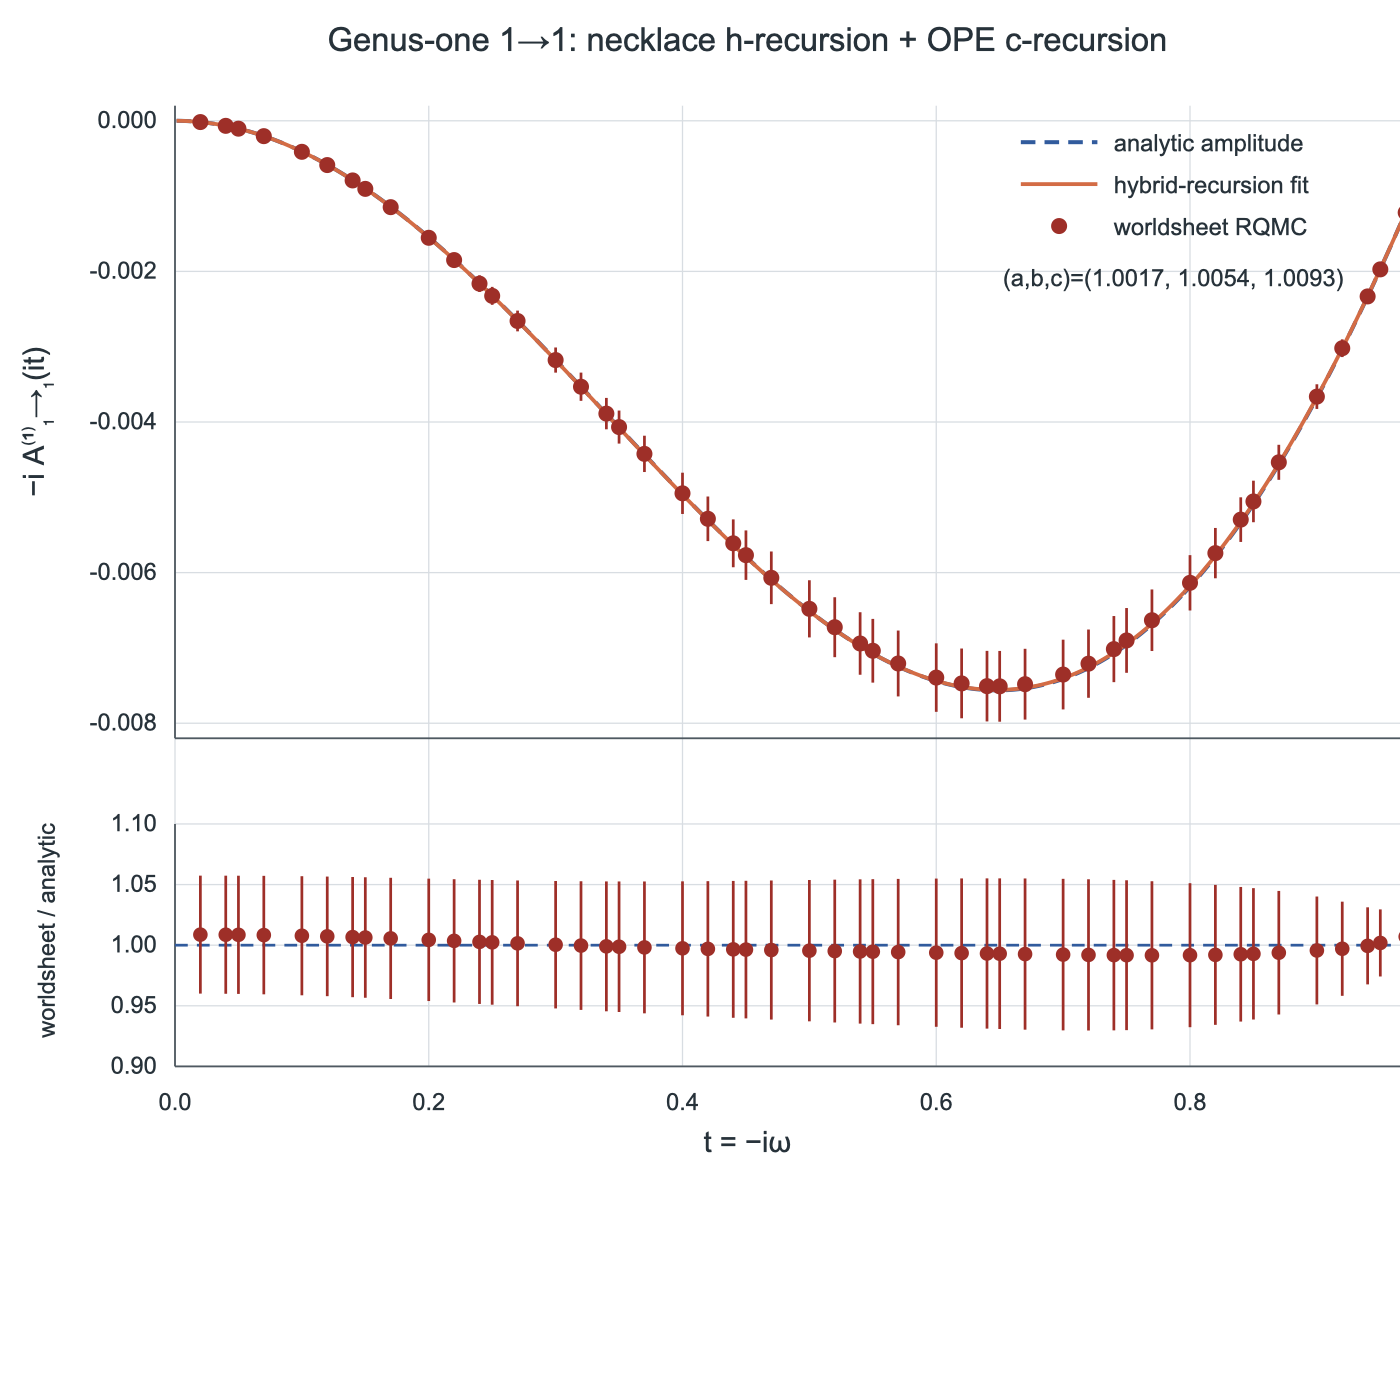
\includegraphics[width=0.96\textwidth]{results/genus1_two_point_worldsheet/imaginary_hybrid_hc_t_scan10_n256_v2/genus1_two_point_hybrid_recursion.png}
\caption{Current fifty-point genus-one $1\to1$ result.  The upper panel
shows the native worldsheet data after the BRY map, the hybrid-recursion fit,
and the exact matrix-model prediction.  The lower panel shows the pointwise
ratio.  Error bars are RQMC-only and are correlated through four shared
scrambles.}
\label{fig:two-point-result}
\end{figure}
\FloatBarrier

\section{Interpretation and limitations of the
\texorpdfstring{$1\to1$}{1 to 1} result}
\label{sec:two-point-limitations}

The fifty-point curve is an audited numerical worldsheet result, not an exact
evaluation of the generic torus integral.  Its displayed errors measure the
scatter of four shared RQMC replicas.  They exclude possible systematic
effects from finite block orders, momentum cutoff and quadrature, the
leading-disc approximation, and the three-term cusp ansatz.  The direct
fallback and channel audits control the conformal-block implementation, while
the full energy dependence gives a stringent global check.

The supported conclusions are:
\begin{enumerate}
  \item the native worldsheet points reproduce the analytic genus-one shape
  across the convergent imaginary-energy strip;
  \item the fitted normalization and three shape coefficients are consistent
  with the exact matrix-model value one;
  \item the current central fit is closer to the exact polynomial than the
  BRY central fit, but the difference is not significant at the present RQMC
  precision;
  \item a future precision claim should increase the number of independent
  shared scrambles and vary momentum, collision, block, and tail designs
  together;
  \item extending through $t>1$ requires the correct OPE-channel crossed-pole
  residue, or a necklace-channel implementation valid there.
\end{enumerate}

No conclusion about higher torus amplitudes follows from the two-point
calculation alone.  The current three-point result below is an independent
six-real-dimensional moduli integration and is not inferred from this fit.

\section{Current torus three-point result: genus-one
\texorpdfstring{$1\to2$}{1 to 2}}
\label{sec:three-point}

\subsection{Blind kinematics and integral}

The symmetric imaginary-energy slice is
\begin{equation}
 \omega=\ii t,
 \qquad
 \omega_1=\omega_2=\frac{\ii t}{2},
 \qquad 0<t<1.
 \label{eq:three-point-kinematics}
\end{equation}
This is the convergent pole-free chamber: no DOZZ pole crosses a positive-real
Liouville-momentum contour.  Both outgoing positions are integrated over the
full torus.  In the necklace chart they are sorted along the cylinder and the
three contracting gaps are
\begin{equation}
 \log q_0=\ii w_{(1)},
 \qquad
 \log q_1=\ii\bigl(w_{(2)}-w_{(1)}\bigr),
 \qquad
 \log q_2=\ii\bigl(2\pi\tau-w_{(2)}\bigr).
 \label{eq:three-point-gaps}
\end{equation}
Consequently $q_0q_1q_2=\exp(2\pi\ii\tau)$ pointwise.  The Liouville
correlator is a threefold positive-momentum integral with measure
$dQ_0dQ_1dQ_2/\pi^3$ and three DOZZ coefficients.  No matrix-model expression
enters this kernel or the Cannon worker code.

\subsection{Current \texorpdfstring{$h$}{h}-recursion-dominant channel atlas}

Most moduli points are evaluated in the necklace chart.  Each cylinder
variable is mapped to its elliptic nome $\widehat q_a=E(q_a)$.  The edge with
largest $|\widehat q_a|$ is expanded adaptively to the smallest order $N$
satisfying
\begin{equation}
 |\widehat q_a|^{N+1}\leq5\times10^{-5},
 \label{eq:three-point-order-rule}
\end{equation}
with a floor of 3 and a prepared cap of 8; the other two edges are kept
through order 3.  The largest and second-largest necklace nomes encountered
are $0.183754$ and $0.049936$.  For every value of $t$, the selected orders are
\begin{equation}
 N=3:4076,
 \qquad N=4:19,
 \qquad N=5:1,
 \qquad N=6,7,8:0.
\end{equation}

The simultaneous internal-weight recursion is regulated by
$2F(25+\epsilon)-F(25+2\epsilon)$ with $\epsilon=0.025$.  The common eta
vacuum factor is cancelled algebraically against the Liouville primary vacuum
factor before exponentiation.  If the best necklace nome exceeds $0.30$, or
the second-best exceeds $0.07$, a local pair- or comb-OPE chart is used
instead.  Those OPE blocks use fixed-weight $c$-recursion in their natural
conformal frame, including the required frame factor.  The largest OPE nome
actually sampled is $0.067143$, and no $c$-recursion collision occurs.

The current atlas therefore makes $h$-recursion the dominant method while
reserving $c$-recursion for a small region.  Per value of $t$, the recorded
channel counts are 4096 necklace, 42 pair-OPE, and 336 comb-OPE evaluations.
Their contributions to the final integral range over $70.98$--$72.21\%$,
$14.81$--$19.38\%$, and $9.65$--$13.02\%$, respectively.

\subsection{Frozen ten-point worldsheet scan}

All ten points use one exact numerical design:
\begin{itemize}
  \item four aligned scrambled Sobol replicas with $2^8=256$
  six-dimensional points in every channel stratum;
  \item direct integration of the compact region through $\tau_2=8$ and an
  importance-sampled tail from $\tau_2=8$ to infinity, with proposal exponent
  $3/2$;
  \item three distinct but equivalent power--Legendre maps on
  $0\leq Q\leq5$, each of order 8;
  \item necklace orders $N_{\rm high}=8$ and $N_{\rm low}=3$, local OPE
  order 6, loop orders 4 and 2, patch radius $0.15$, and triple-patch radius
  $0.10$.
\end{itemize}

The assembled Cannon output contains nine new shards and reuses the existing
$t=0.75$ point only after exact-design and hash validation.  Table
\ref{tab:three-point-scan} is the complete current result.

\begin{table}[htbp]
\centering
\caption{Current frozen target-blind torus three-point scan.  The displayed
error is the standard error of four aligned RQMC scrambles.  The tail is
integrated directly to infinity rather than fitted from fixed-height slices.}
\label{tab:three-point-scan}
\small
\begin{tabular}{r r r r}
\toprule
$t$ & $-\operatorname{Im}\cI_{1,3}$ & RQMC SE & tail fraction\\
\midrule
0.05 & 0.0000281249 & 0.0000043727 & $8.71\%$\\
0.15 & 0.000729587  & 0.000113149  & $8.48\%$\\
0.25 & 0.00312010   & 0.000480503  & $8.18\%$\\
0.35 & 0.00759257   & 0.00115398   & $7.87\%$\\
0.45 & 0.01368245   & 0.00203629   & $7.60\%$\\
0.55 & 0.02008363   & 0.00289831   & $7.39\%$\\
0.65 & 0.02486229   & 0.00343811   & $7.23\%$\\
0.75 & 0.02581783   & 0.00337249   & $7.11\%$\\
0.85 & 0.02093083   & 0.00253755   & $7.03\%$\\
0.95 & 0.00885084   & 0.000973781  & $6.98\%$\\
\bottomrule
\end{tabular}
\end{table}

The curve rises from zero, has its largest sampled value at $t=0.75$, and
falls toward $t=1$.  A target-free quadratic through
$t=0.65,0.75,0.85$ gives
\begin{equation}
 \boxed{t_{\rm peak}^{\rm ws}=0.7164\pm0.0029}
 \qquad\text{(aligned-scramble RQMC only)}.
 \label{eq:three-point-worldsheet-peak}
\end{equation}
The relative RQMC errors decrease from $15.5\%$ at $t=0.05$ to $11.0\%$ at
$t=0.95$.  The direct tail contributes $6.98\%$--$8.71\%$.  These errors do
not include a calibrated momentum-, block-, atlas-threshold-, or
tail-proposal systematic.

\subsection{Post-freeze comparison with the matrix model}

The ten-point worldsheet manifest was first hash-frozen on Cannon.  Its
target-free local shape analysis was then independently frozen before the
genus-one stripped matrix polynomial from Eq.~(2.55) of
Collier--Eberhardt--Rodriguez~\cite{CER} was evaluated:
\begin{equation}
 \widehat S_{1,3}
 =-\frac{(\omega_1+\omega_2-\ii)(\omega_1+\omega_2-2\ii)}{48}
 \left(\omega_1^2-\ii\omega_1+\omega_2^2-\ii\omega_2+1\right).
 \label{eq:three-point-matrix-polynomial}
\end{equation}
The stable three-point normalization already fixed at genus zero gives
$F_0=\omega\omega_1\omega_2$.  CER expand their amplitudes using
$g_s^{\mathrm{CER}}=\sqrt{2}/\mu$, whereas the present expansion variable is
$g_\mu=\mu^{-1}=2\pi g_s$.  The genus-one/tree ratio therefore contains
$(g_s^{\mathrm{CER}}/g_\mu)^2=2$, so that
\begin{equation}
 F_1^{\mathrm{MM}}=2F_0\widehat S_{1,3}.
 \label{eq:three-point-cer-to-bry}
\end{equation}
On the equal imaginary ray this gives
\begin{equation}
 F_1^{\mathrm{MM}}(t)
 =-\frac{\ii t^3(t-1)(t-2)(1+t-t^2/2)}{96}.
 \label{eq:three-point-equal-ray}
\end{equation}
Equivalently, in the native ordinate shown in Table
\ref{tab:three-point-comparison},
\begin{equation}
 -\operatorname{Im}\cI_{1,3}^{\mathrm{MM}}(t)
 =\frac{\pi t^3(t-1)(t-2)(1+t-t^2/2)}{24}.
\end{equation}

\begin{table}[htbp]
\centering
\caption{Comparison evaluated only after the target-blind scan and shape
analysis were frozen.  Pulls use the pointwise RQMC standard errors only.}
\label{tab:three-point-comparison}
\small
\begin{tabular}{r r r r}
\toprule
$t$ & $-\operatorname{Im}\cI_{1,3}^{\mathrm{MM}}$
& worldsheet / MM & RQMC pull\\
\midrule
0.05 & 0.0000317891 & 0.8847 & $-0.838$\\
0.15 & 0.000791100  & 0.9222 & $-0.544$\\
0.25 & 0.00327169   & 0.9537 & $-0.315$\\
0.35 & 0.00775727   & 0.9788 & $-0.143$\\
0.45 & 0.01371520   & 0.9976 & $-0.016$\\
0.55 & 0.01987684   & 1.0104 & $+0.071$\\
0.65 & 0.02443801   & 1.0174 & $+0.123$\\
0.75 & 0.02534664   & 1.0186 & $+0.140$\\
0.85 & 0.02064459   & 1.0139 & $+0.113$\\
0.95 & 0.00883076   & 1.0023 & $+0.021$\\
\bottomrule
\end{tabular}
\end{table}

All ten worldsheet points lie within one pointwise RQMC standard error of the
matrix curve.  The largest absolute pull is $0.838$, and the ratios range from
$0.8847$ to $1.0186$.  The matrix curve peaks at $t\simeq0.720$, consistent
with Eq.~\eqref{eq:three-point-worldsheet-peak}.  Since the ten estimates use
only four aligned scrambles, the covariance matrix has low rank and no joint
goodness-of-fit significance is assigned.  No calibrated truncation
systematic has been added to the displayed errors.

\begin{figure}[htbp]
\centering
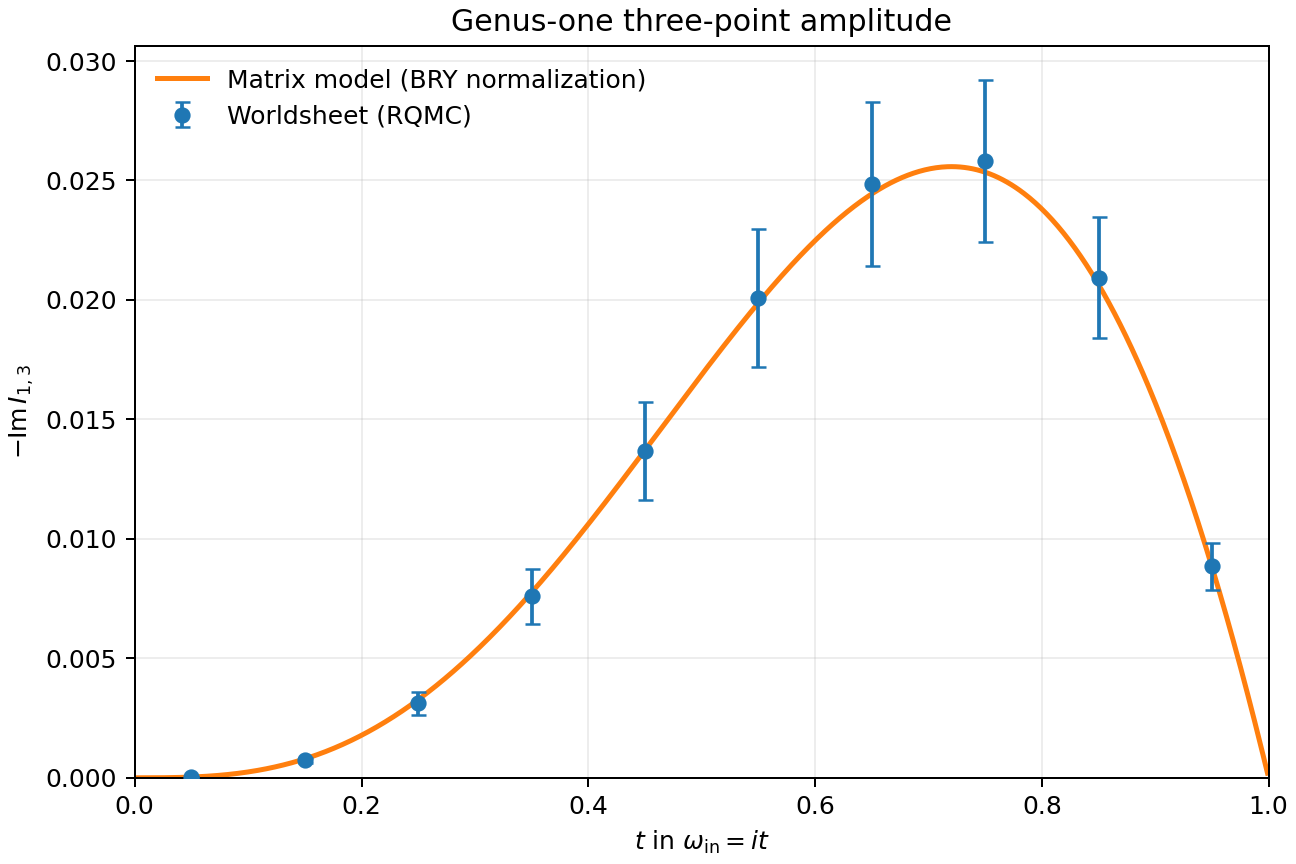
\includegraphics[width=0.92\textwidth]{results/genus1_three_point_worldsheet/hdominant_scan10_p8_h8l3_q030_007_n256_r4_v1/assembled/worldsheet_vs_matrix_bry.png}
\caption{Current genus-one $1\to2$ result on the equal imaginary-energy ray.
The blue worldsheet estimates are shown as unconnected points with RQMC error
bars.  The orange matrix-model curve is evaluated only after the worldsheet
scan and target-free shape analysis were frozen.}
\label{fig:three-point-result}
\end{figure}
\FloatBarrier

\section{Error budget and next gates}
\label{sec:error-budget}

For every future torus $1\to n$ production point, the following uncertainties
should be retained separately:
\begin{enumerate}
  \item adjacent momentum rules and changes of the high-momentum cutoff;
  \item adjacent Virasoro-block orders and direct-sewing fallback counts;
  \item moduli RQMC depth and additional independent scrambles;
  \item agreement between overlapping necklace and OPE channels;
  \item collision-disc radius and analytic leading-disc approximation;
  \item direct-tail proposal exponent, tail boundary, and independent
  tail-stratum depth;
  \item distance to the next Liouville-momentum contour wall and any crossed
  residue contribution.
\end{enumerate}
The current $1\to1$ evidence identifies the analytic answer strongly in the
controlled imaginary-energy chamber.  The current $1\to2$ points agree with
the BRY-normalized matrix curve at their RQMC precision, but the absence of a
calibrated momentum-, block-, atlas-, and tail-proposal systematic prevents a
precision discrepancy claim or a general torus-amplitude inference.

\appendix
\section{Machine-readable provenance and implementation map}
\label{sec:code-map}

This appendix is a reviewer-oriented map of the code and frozen artifacts
that support the torus $1\to n$ claims.  File names are relative to the
repository root unless stated otherwise.

\subsection{Trust boundary used in the blind calculations}

The production flow is deliberately split into files with different
authority:
\begin{enumerate}
  \item a worldsheet kernel evaluates Liouville structure constants,
  timelike factors, conformal blocks, and moduli weights;
  \item a target-blind scan produces raw worldsheet integrals and numerical
  diagnostics but contains no matrix-model polynomial;
  \item the source JSON files are hashed and frozen in a manifest;
  \item only a separate post-freeze fitter or comparison file applies the BRY
  convention map or evaluates the matrix-model function.
\end{enumerate}

\subsection{Torus \texorpdfstring{$1\to1$}{1 to 1} code path}

\begin{description}[style=nextline,leftmargin=3.8cm]
  \item[Worldsheet kernel]
  \path{plumbing/genus1_two_point_worldsheet.py} implements the native torus
  integrand, hybrid channel selection, and block backends.

  \item[RQMC production]
  \path{plumbing/integrate_genus1_two_point_worldsheet.py} implements the
  finite-cutoff moduli integration and cusp fit;
  \path{plumbing/run_genus1_two_point_imaginary_scan.py} runs the target-blind
  imaginary-ray scan.

  \item[Block audit]
  \path{plumbing/genus1_two_point_hybrid_recursion_report.md} records the
  necklace $h$-recursion, OPE $c$-recursion, coincident-weight limits, and
  direct-descendant validation.  The complete direct anchor is
  \path{plumbing/results/genus1_two_point_worldsheet/direct_current_t045_n256_v1.json}.

  \item[Later fit and plot]
  \path{plumbing/fit_genus1_two_point_bry_scan.py} reads only frozen native
  artifacts before applying the BRY map;
  \path{plumbing/plot_genus1_two_point_hybrid_recursion.py} produces
  Figure~\ref{fig:two-point-result}.
\end{description}

The principal $1\to1$ artifacts are
\begin{itemize}
  \item
  \path{plumbing/results/genus1_two_point_worldsheet/imaginary_hybrid_hc_t_scan10_n256_v2/worldsheet_scan_manifest.json};
  \item
  \path{plumbing/results/genus1_two_point_worldsheet/imaginary_hybrid_hc_t_scan10_n256_v2/bry_postfreeze_fit_50point.json};
  \item
  \path{plumbing/results/genus1_two_point_worldsheet/imaginary_hybrid_hc_t_scan10_n256_v2/genus1_two_point_hybrid_recursion.png}.
\end{itemize}

\subsection{Torus \texorpdfstring{$1\to2$}{1 to 2} code path}

\begin{description}[style=nextline,leftmargin=3.8cm]
  \item[Three-edge block]
  \path{plumbing/torus_three_point_blocks.py} implements generic three-edge
  blocks and exact $c=25$ sewing;
  \path{plumbing/torus_two_point_blocks.py} supplies the $N$-dimensional
  elliptic-nome re-expansion.

  \item[Worldsheet kernel and atlas]
  \path{plumbing/genus1_three_point_worldsheet.py} implements the target-free
  three-point kernel;
  \path{plumbing/genus1_three_point_channel_atlas.py} implements the
  $h$-dominant necklace/pair-OPE/comb-OPE atlas;
  \path{plumbing/smoke_genus1_three_point_channel_atlas.py} implements the
  stratified six-dimensional bulk and direct-tail RQMC.

  \item[Checks]
  \path{plumbing/genus1_three_point_worldsheet_checks.py} checks the block and
  geometry;
  \path{plumbing/genus1_three_point_matrix_comparison_checks.py} checks only
  the separate post-freeze comparison formulas.

  \item[Cannon scan and assembly]
  \path{plumbing/run_genus1_three_point_hdominant_scan.py} fixes the exact
  ten-point design and reuse policy;
  \path{plumbing/genus1_three_point_hdominant_cannon.py} prepares and verifies
  the blind shards and writes the first worldsheet freeze.

  \item[Blind analysis and later comparison]
  \path{plumbing/analyze_genus1_three_point_hdominant_scan.py} verifies every
  frozen hash, writes and hashes the target-free shape analysis, and only
  after that second freeze evaluates the BRY-normalized comparison.
\end{description}

The only current $1\to2$ result directory used in this note is
\begin{center}
\small
\path{plumbing/results/genus1_three_point_worldsheet/hdominant_scan10_p8_h8l3_q030_007_n256_r4_v1/}.
\end{center}
Its principal assembled artifacts are
\begin{itemize}
  \item \path{assembled/worldsheet_scan_manifest.json};
  \item \path{assembled/worldsheet_freeze_manifest.json};
  \item \path{assembled/worldsheet_shape_analysis_blind.json};
  \item \path{assembled/worldsheet_analysis_freeze_manifest.json};
  \item \path{assembled/matrix_comparison_after_blind_freeze.json};
  \item \path{assembled/worldsheet_vs_matrix_bry.png}.
\end{itemize}

\subsection{Recommended faithfulness-review order}

The shortest review path that checks every conceptual boundary is:
\begin{enumerate}
  \item verify the sewing normalization and BRY coupling dictionary;
  \item inspect the two-point hybrid-recursion audit and its direct anchor;
  \item verify the fifty source hashes in the canonical manifest;
  \item confirm by source inspection that the scan files contain no target
  polynomial;
  \item reproduce the post-freeze fifty-point fit and plot;
  \item inspect the three-edge block checks, channel atlas, and sorted-cylinder
  geometry;
  \item verify all ten three-point shard hashes and the first worldsheet freeze;
  \item reproduce the target-free shape analysis and verify its second freeze;
  \item only then inspect the post-freeze BRY comparison.
\end{enumerate}

Each amplitude section contains only its latest audited result.  This note
should next be extended by convergence variations of the current $1\to2$
design or by the first torus $1\to3$ integration.

\clearpage
\begin{thebibliography}{9}

\bibitem{BRY}
B.~Balthazar, V.~A.~Rodriguez, and X.~Yin,
``The $c=1$ String Theory S-Matrix Revisited,''
\href{https://arxiv.org/abs/1705.07151}{arXiv:1705.07151}.

\bibitem{CER}
S.~Collier, L.~Eberhardt, and V.~A.~Rodriguez,
``$c=1$ Strings as a Matrix Integral,''
\href{https://arxiv.org/abs/2604.06301}{arXiv:2604.06301}.

\end{thebibliography}

\end{document}
